\documentclass{article}
\usepackage[utf8]{inputenc}

\title{Notes on paper Tesis UFRO}
\author{Juan P. Gil }
\date{May 2018}

\usepackage{natbib}
\usepackage{graphicx}

\begin{document}

\maketitle

\begin{abstract}
Notes towards make the article to be sent as part of the Master Degree.
\end{abstract}


% \begin{figure}[h!]
% \centering
% 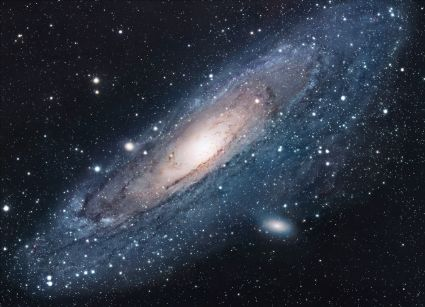
\includegraphics[scale=1.7]{universe}
% \caption{The Universe}
% \label{fig:universe}
% \end{figure}


\section{Introduction}

Hardware and software at observatory facilities.

General information regarding the log analysis.

Proposal: generate a set of features from event logs to describe time intervals.

Goals of the work: to detect outliers.

framework of the problem, state of the art, uses of the applied technique
classical approaches, paper proposal. Goals of the study
Organization of the rest of the paper


\section{Data Source}


\subsection{Logs at ALMA}

\subsection{Log Recollection}

log rate generation


\subsection{Cases definition}
Events generated by antennas

how to extract the value to study

-- train and test sets



\section{Method}

\subsection{Extraction of Time Intervals}

Definitions.

Action. Event. Log. 

Traces. 

Pairs (subset of AxA)

Log Partitioning.

Extract time intervals.

\subsection{Analysis of Time Intervals}

The Serial Case

Correlations. 

Introducing Parallelism

Random Traces

\subsection{Implementation of the Algorithm}

Order, steps, performance


\section{Simulated Event Logs}

Parameters: activities, serial to parallel, log size

comparison with other methods

\subsection{Synthetic Generator}



\section{Case Study: Antenna operation}

results by the method
domain expert analysis
parameter calibration

\section{Conclusion}

``I always thought something was fundamentally wrong with the universe'' \citep{adams1995hitchhiker}


\bibliographystyle{plain}
\bibliography{references}
\end{document}

